\documentclass[conference,flushend]{iaria} % (based on IEEEtran.cls)
% The class iaria.cls loads biblatex/biber with correct IARIA settings
% as well as a set of common packages (times, inputenc[utf8], fontenc[T1],
% graphicx, xcolor, url, orcidlink, hyperref, extdash[shortcuts])

\usepackage{subfigure}
\usepackage{csquotes}
\usepackage{svg}
\usepackage{float}

\newcommand*{\captionsource}[2]{%
  \caption[{#1}]{%
    #1%
    \\\hspace{\linewidth}%
    \textbf{Source:} #2%
  }%
}

\addbibresource{references.bib}
\title{Fast Charging Communication and Cybersecurity: A Technology Review}
\author{
  \IEEEauthorblockN{%
    Jakob Löw\orcidlink{0009-0006-7088-8684}, Kevin Mayer\orcidlink{0000-0002-5597-3913}, Hans-Joachim Hof\orcidlink{0000-0002-6930-9271}}
  \IEEEauthorblockA{%
    CARISSMA Institute of Electric, Connected and Secure Mobility \\
    University of applied sciences Ingolstadt \\
    Ingolstadt, Germany \\
    e-mail: {\tt$\lbrace$jakob.loew\,|\,kevin.mayer\,|\,hof$\rbrace$@thi.de}
} }
\begin{document}
\maketitle
\begin{abstract}
With the increasing amounts of electric vehicles on the road, the demand for public charging stations increases as well.
While AC charging is used for charging at home, DC fast charging is commonly used when traveling long distances.
Since DC fast charging requires higher level communication between vehicle and charging station, it provides an increased attack surface to both sides.
This paper reviews communication standards and their implementations used in fast charging scenarios.
Focusing on the cybersecurity aspects of these communications, we review and sketch up new mechanisms for attacking charging station communication.
\end{abstract}
\begin{IEEEkeywords}
charging; fast charging; ccs; iso15118; DC charging; electric vehicle; vehicle charging.
\end{IEEEkeywords}

\section{Introduction}
Many countries are currently transitioning away from combustion engine vehicles towards battery electric ones.
This transition is happening at a rapid rate, because buying an electric vehicle often gets incentivised through tax reductions or straight refunds \cite{kraftfahrtbundesamt_anzahl_2024}.
With people buying more and more electric vehicles, the demand for charging infrastructure rises.
In Germany not only electric vehicles, but also the buildup of charging infrastructure got heaviliy subsidized by the government.
This high demand and government incentives resulted in a rapid growth in charging station numbers, suppliers and operators \cite{bundesnetzagentur_anzahl_2024}.
Due to the rushed development, the cybersecurity of current charging stations is below average compared to other cyberphysical systems \cite{nasr_power_2022, johnson_review_2022, ahalawat_security_2022}.
Recently cybersecurity researchers investigating charging backend infrastructure have found a range of text book vulernabilities, such as SQL injection, cross site scripting or unauthenticated remote update procedures \cite{nasr_power_2022}.
\\
This paper will focus on fast charging stations. Because of their functionality design, described in a later section, they require a high level direct communication with the vehicle for charging conditions and limits.
While other works such as Tu et al. \cite{tu_extreme_2019} have already covered eletrical and other aspects of fast charging stations, this paper will focus on communication aspects.
The ISO15118 standard was created for communication between charging stations and vehicles, enabling interoperability between stations and vehicles from different manufacturers.
This high level communication protocol provides a larger attack surface compared to other charging techniques, making it more interesting for cybersecurity reserarch.

\section{Charging Station Communication}
Electricity generally comes in two forms: alternating current (AC) and direct current (DC).
While power grids are usually AC, batteries need to be charged using DC.
Therefore the AC needs to be converted to DC either in the car or in the charging station itself.
While cars usually come with an onboard AC to DC converter for charging the onboard battery their power is usually limited between 7 and 22 kW.
In order to achieve higher charging powers, a fast charging station provides a stationary AC to DC converter. Placing it outside of the car removes weight requirements, simplifies cooling and thus allows higher charging currents. \\
In general charging stations can be divided into three categories:
\begin{enumerate}
\item Unmetered AC charging (often used in residential buildings)
\item Commercial AC charging stations
\item DC fast charging stations
\end{enumerate}%
%
The following subsections describe the communication and payment mechanisms of these three kinds of charging stations as well as the included security concepts.

\subsection{Low Level Communication}
AC charging stations usually supply grid power directly, making them just sockets with some very basic communication to the vehicle.
In the early days of electric vehicle adoption mainly these kind of charging stations were built.
Because charging a modern vehicle using an AC charging station can take multiple hours, they usually aren't used for long distance driving.
Because of their low price and low electrical requirements they are however still widely used and newly installed, especially for home and office charging as well as on park and ride parking lots. \\
The by far most common plug for AC charging is the type 2 connector shown in figure \ref{fig:type2}. It is used not only the standard charging plug in Europe, but also in China and other parts of Asia.
Apart from the typical connections of a 3-phase power socket, the connector incorporates two additional pins: charge pilot (CP) and proximity pilot (PP).
These two pins are used for a very simple resistor based signaling scheme defined in IEC 61851 \cite{iec_iec_2010} and explained by \cite{dalheimer_ladeinfrastruktur_2017}:
The charging cable includes a resistor between proximity pilot and protective earth (PE), which signals the maximum current for this cable.
The charging station supplies a +12V/-12V pulse width modulation (PWM) signal between CP and PE.
The vehicle contains both a diode and a resistor between CP and PE, such that the charging station can detect the presence of a vehicle based on the negative voltage being dropped by the diode and the positive voltage being reduced by the resistor.
As soon as the vehicle is ready to charge it connects a second resistor between CP and PE further reducing the voltage.
For unmetered AC charging this is sufficient to start a charging session.
For public AC charging infrastructure usually external means of payment, such as mobile app activation or contactless payment have to be used before the charge session is started.
During the charging session the charging station tells the vehicle the maximum allowed current through changing the duty cycle of the +12V/-12V PWM signal between CP and PE.
There exists a special PWM duty cycle of 5\%, which can be used by the charging station to tell the vehicle to use the high level ISO15118 protocol for communication rather than the low level communication described in IEC 61851 \cite{iec_iec_2010}.

\begin{figure}[ht]
    \centering
    \begin{subfigure}
        \centering
        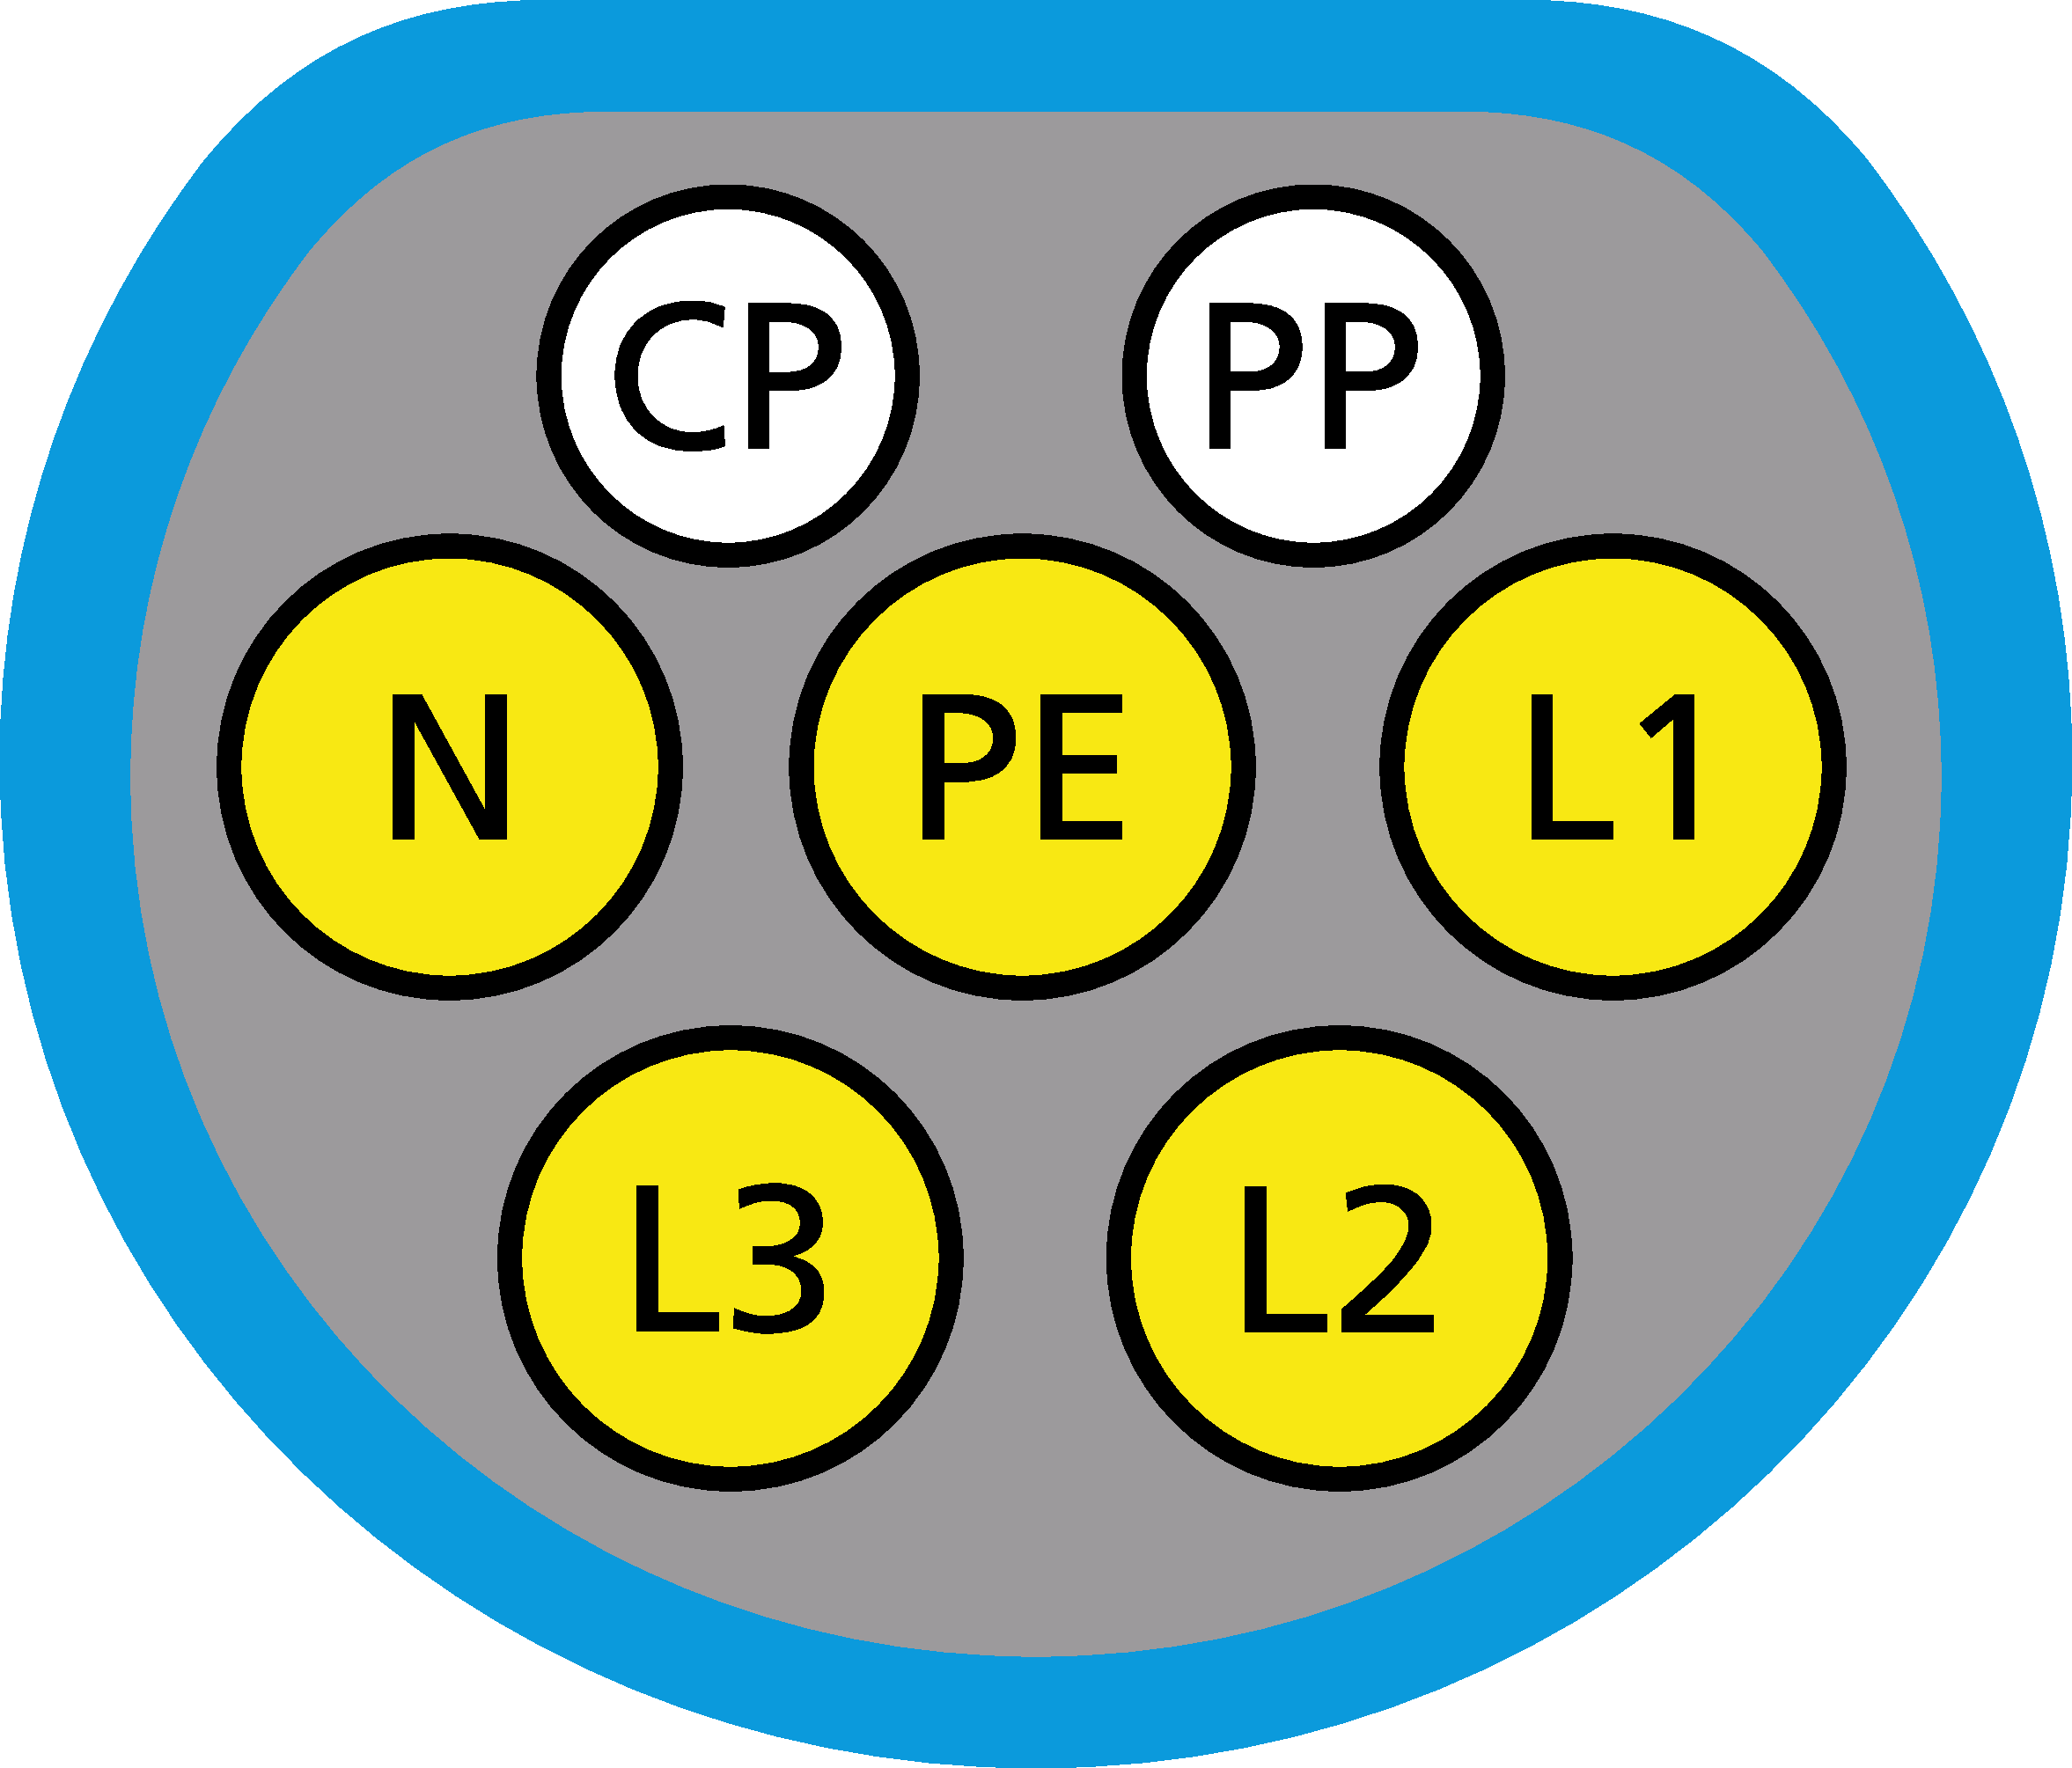
\includegraphics[width=.2\textwidth]{graphs/type2.pdf}
        %\caption{IEC 62196 Type 2 connector schematic}
        \label{fig:type2}
    \end{subfigure}
    \hfill
    \begin{subfigure}
        \centering
        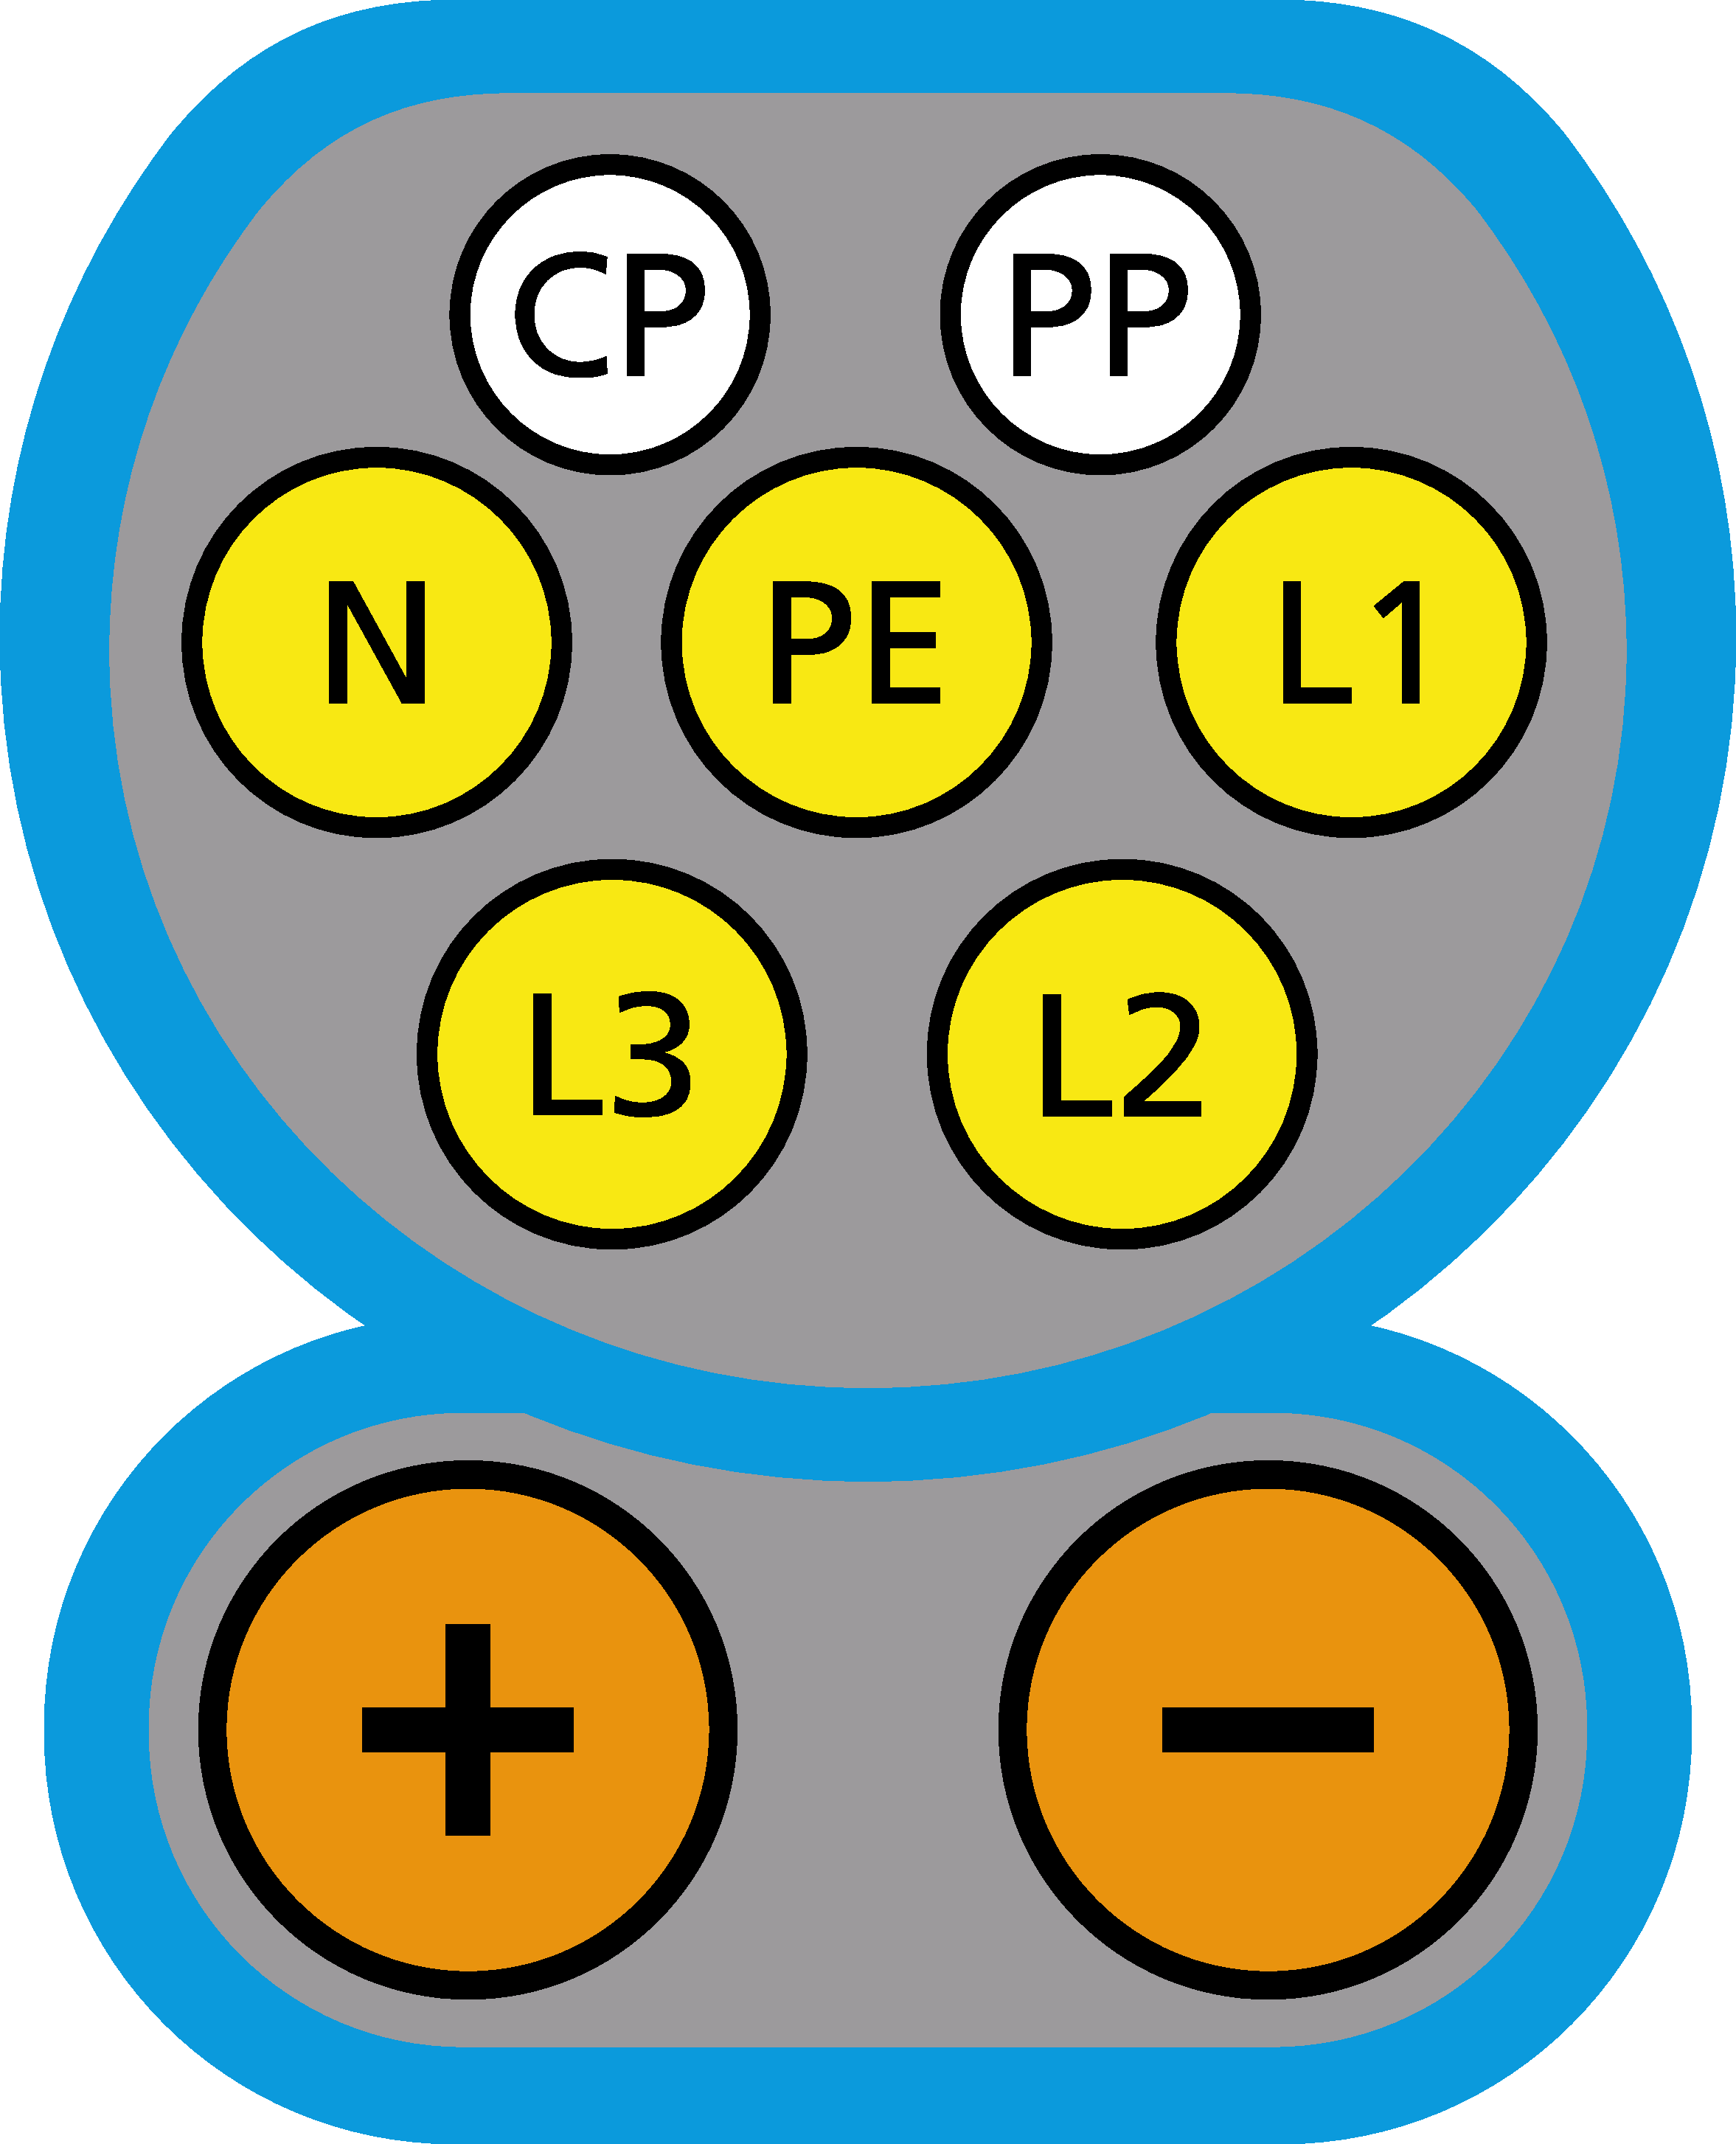
\includegraphics[width=.2\textwidth]{graphs/ccs.pdf}
        %\subcaption{Combined charging system connector schematic}
        \label{fig:ccs}
    \end{subfigure}
    \caption{Schematic diagrams type 2 (left) and combined charging system (right) connectors \cite{chris828_type_2020}}
    \label{fig:connectors}
\end{figure}

% refs:
%% \cite{IEC61851} - resistor & PWM communication
%% \cite{dalheimer_ladeinfrastruktur_2017} - gonium talk about charging stations: TODO often other vulnerabilities
%% nope: \cite{antoun_detailed_2020} - claims grid communication exists, claims home chargers have high-level communication with vehicles

\subsection{High Level Communication}
While charging a vehicle with AC requires little to no communication.
DC charging stations on the other hand are required to communicate to the vehicle for properly supplying the correct voltage and power to the battery.
For this high level communication the industry standard ISO15118 \cite{isoiec_isoiec_2012} was created, enabling interoperability between different vehicle manufacturers and charging station vendors.
The standard is based on more or less common standards for all layers of the OSI model:
After the initial handshake of the low level communication, described in the previous section, is done, the charging station signals the vehicle to use high level communication by supplying a PWM duty cycle of 5\%.
Afterwards a powerline communication is established using the PWM signal between the charge pilot and protective earth as a carrier frequency.
To prevent crosstalk problems \cite{li_crosstalk_2019, theethayi_parameters_2003, ngo_bisse_crosstalk_2023} usually arising with powerline communication, ISO15118-3 \cite{isoiec_isoiec_2012-1} describes \enquote{signal level attentuation characterization} (SLAC).
SLAC measures the interference on the powerline communication line as well as matches vehicles with their nearest charging station connected to the powerline.
Once powerline communication is established IPv6 with link local stateless autoconfiged addresses is used on top for communication between the charging station and the vehicle.
While the ISO15118-2 standard \cite{isoiec_isoiec_2012} itself is based on TCP, first a UDP broadcast service discovery is used for exchanging IPv6 addresses as well as the port to connect to.
Through this TCP connection the actual payloads required for starting a charging session and controlling charging limits is performed.
For encoding payloads on this TCP connection the standard defines a \enquote{vehicle to grid transfer protocol} (V2GTP) packet format, which apart from some metadata contains one large payload blob encoded in the \enquote{efficient XML interchange} (EXI) format. \\
The ISO15118-2 standard defines a list of request messages sent from the vehicle to the charging station and corresponding response messages sent from the charging station to the vehicle.
During charging two packets are used repeatedly: \verb'CurrentDemandReq' and \verb'CurrentDemandRes'.
The first one is sent by the vehicle to request a specific voltage and current flowing into the vehicles battery.
The latter one is sent by the charging station informing the vehicle about currently measured voltage and current as well as the charging stations limits.
For example the car might request a voltage of $369V$ and a maximum current of $400A$ resulting in a desired charging power of $148kW$.
While the voltage has to be met, depending on the charging stations maximum output power the current might be lower than the requested value, resulting in a slower charging speed. \\
Before this main charge loop is started, the vehicle and charging station perform a payment and cable checking and precharging procedure.
Before the vehicle closes the main contactor relay between battery and charge port, the precharging procedure makes sure the voltage present at the cable matches the battery voltage, reducing in rush current and reducing wear on the main contactor relay.
For payment the vehicle first asks the charging station for supported payment methods.
As of today, mostly the \verb'external' payment method is used, which requires the user to pay through an app or contactless payments.
The standard also supports certificate based authentication allowing the car to authenticate itself and start charging directly after the cable has been plugged in.
This use case and its security implications will be covered in the next section.

\subsection{ISO15118 Security Concepts}
While the most commonly used scheme for the charge loop communication is based on plain TCP, the ISO15118 standard also allows to use TLS for encrypted communication.
Using the UDP broadcast packet, the vehicle can signal support for TLS encrypted communication.
If the charging station also supports TLS encryption it signals this to the vehicle in the UDP response including a port to connect to using TLS.
While TLS provides a secure way of communication, it requires a private key infrastructure (PKI) to sign and distribute certificates.
ISO15118 describes a potential layout of this PKI handing out certificates to vehicle manufacturers and charge point operators, but does not name a specific entity managing this PKI.
As of today there are at least four different companies that created a PKI and allow third parties to acquire certificates \cite{charin_charin_nodate, hubject_download_nodate, nexusgroup_identities_nodate, irdeto_irdeto_nodate}.
Normally a certificate authority simply provides certificates for a service provider, for example for a website.
With ISO15118 however, the vehicle requires a matching client certificate to a potential certificate provided by the charging station.
Thus while having multiple certificate authorities is generally a good idea, it creates a maintenance overhead for both vehicle manufacturers and charging station operators.
As of today the vast majority of all charging sessions is started using external authentication rather than plug and charge.
While PnC promises to improve usability and thus overall technology acceptance, the nature of the TLS implementation details set by the ISO15118 charging standard hinder its spread and is thus rarely used today.
% TODO: move PKI problems and TLS-downgrade to a different section?

\begin{figure*}[ht]
    \centering
    \begin{subfigure}
        \centering
        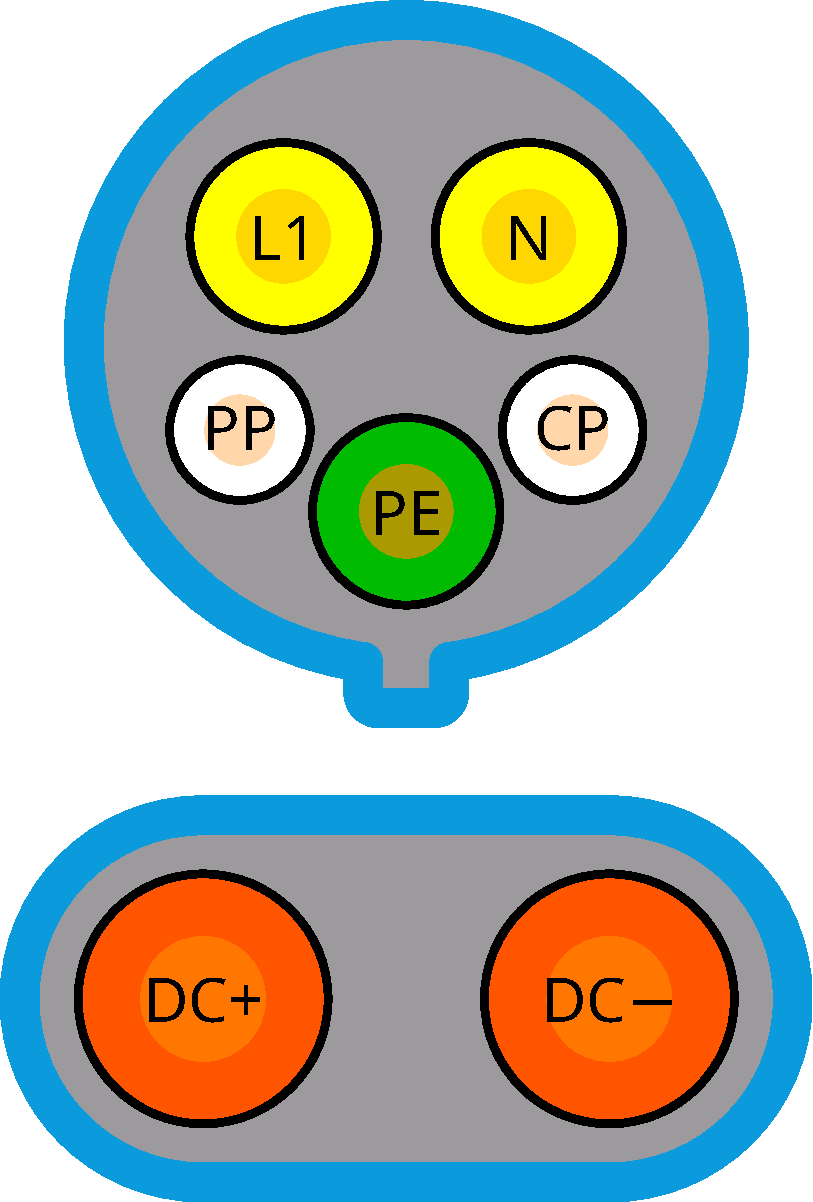
\includegraphics[width=.17\textwidth]{graphs/type1-ccs}
        %\caption{IEC 62196 Type 2 connector schematic}
        \label{fig:type2}
    \end{subfigure}
    \hfill
    \begin{subfigure}
        \centering
        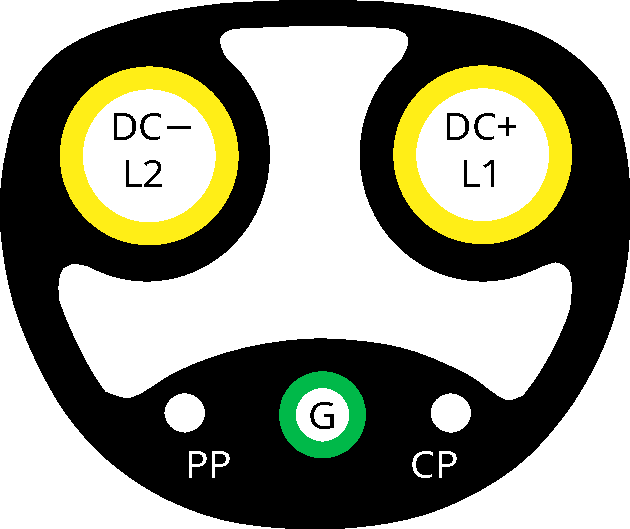
\includegraphics[width=.17\textwidth]{graphs/nacs}
        %\subcaption{Combined charging system connector schematic}
        \label{fig:ccs}
    \end{subfigure}
    \hfill
    \begin{subfigure}
        \centering
        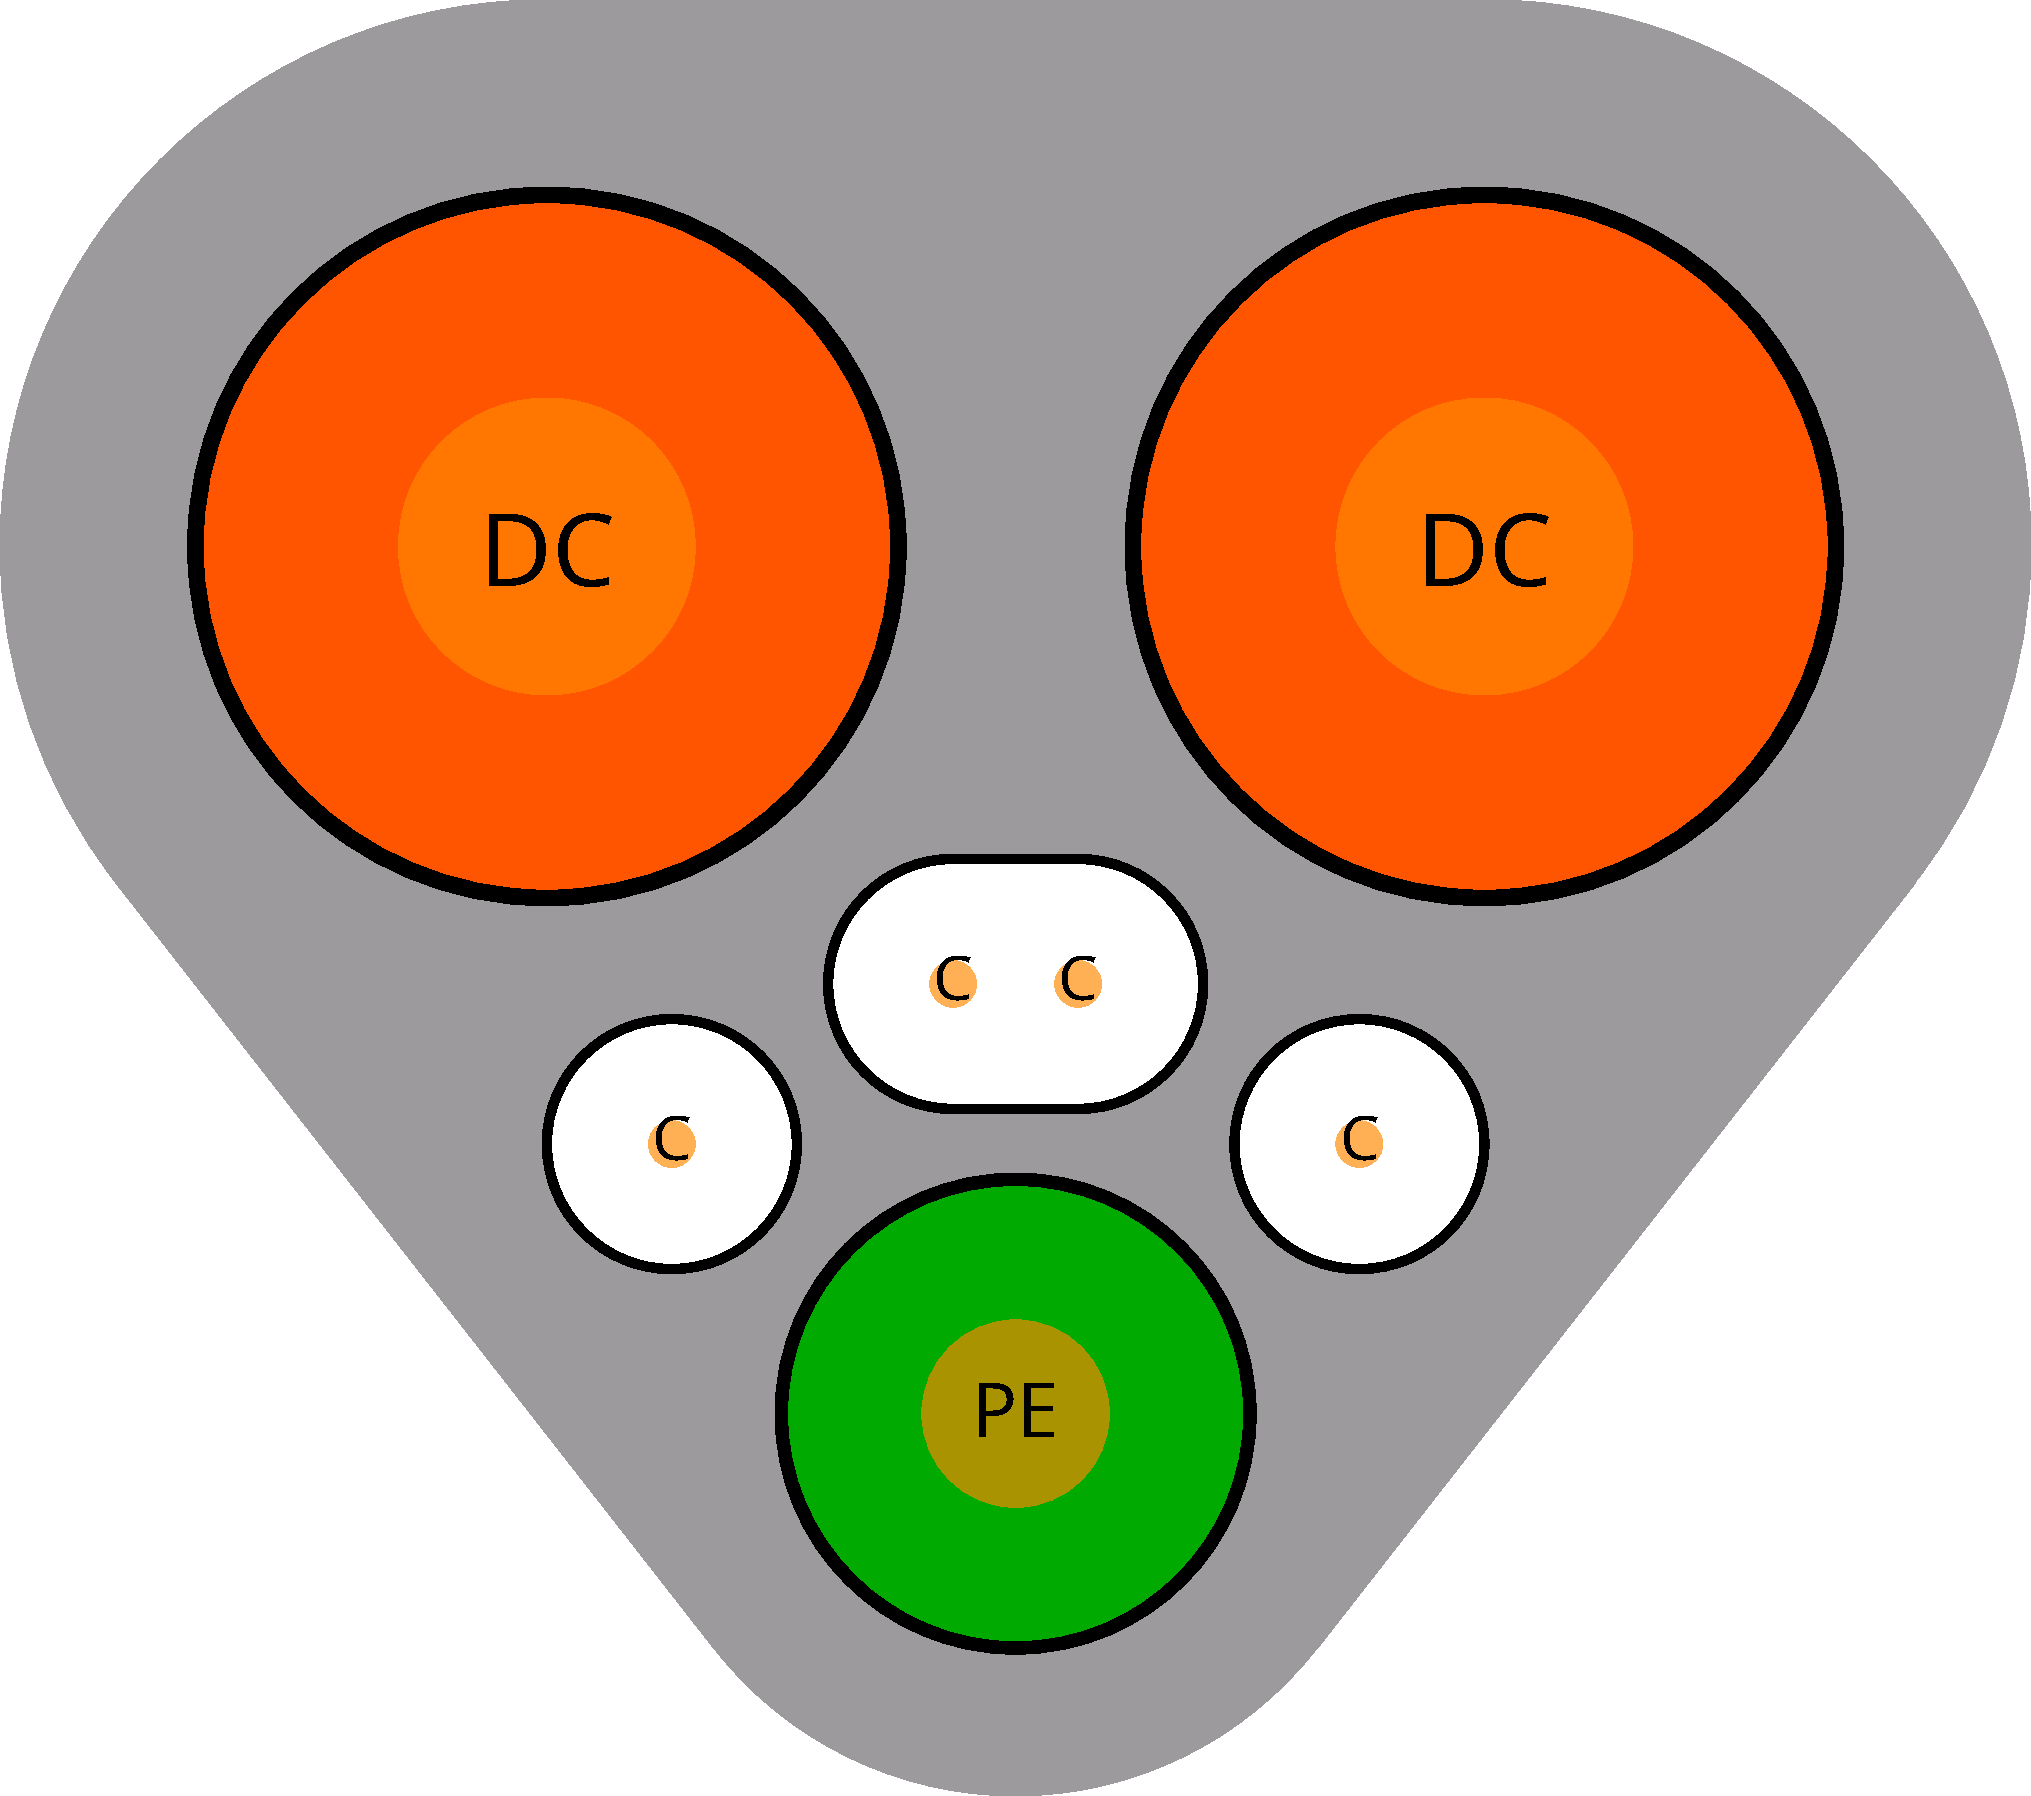
\includegraphics[width=.17\textwidth]{graphs/mcs}
        %\subcaption{Combined charging system connector schematic}
        \label{fig:ccs}
    \end{subfigure}
    \hfill
    \begin{subfigure}
        \centering
        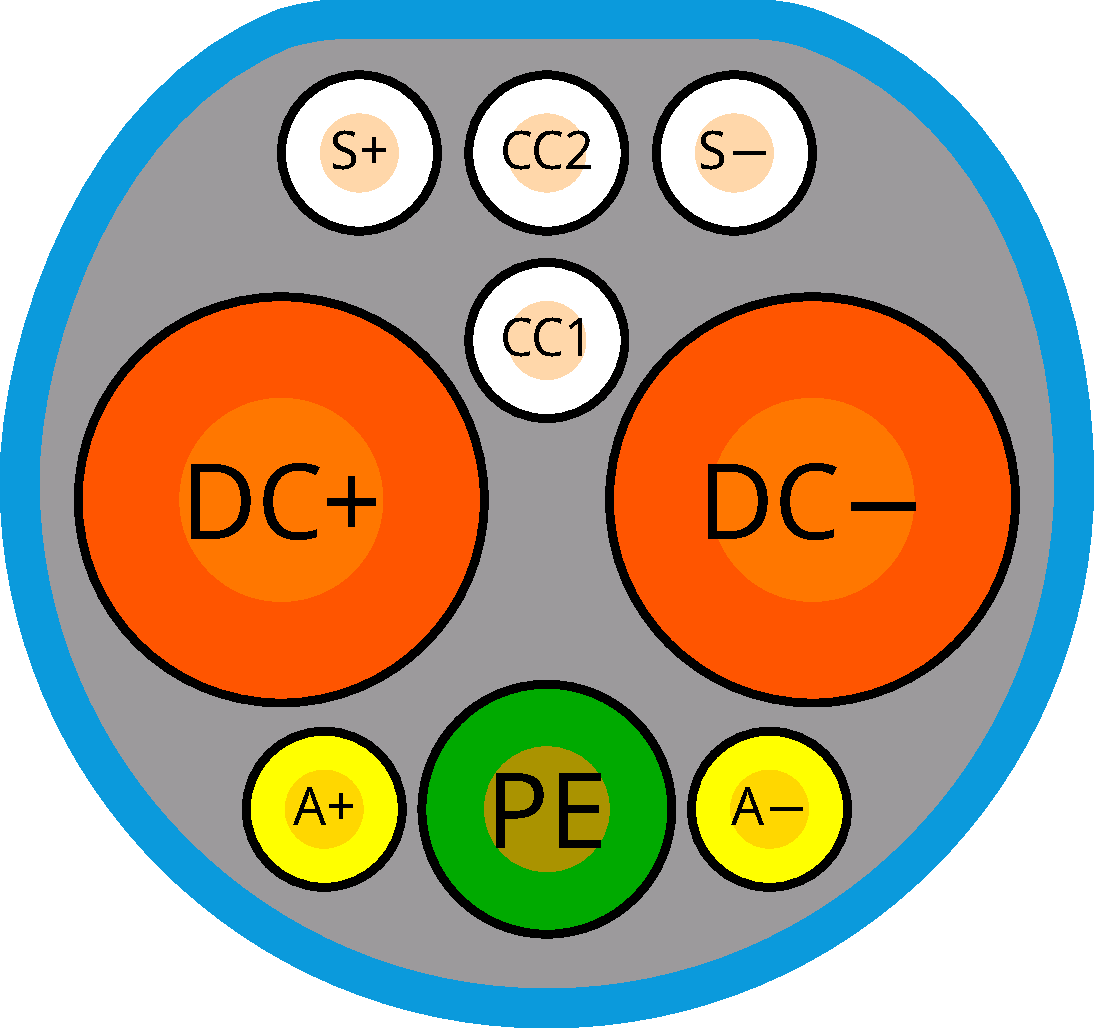
\includegraphics[width=.17\textwidth]{graphs/gbt}
        %\subcaption{Combined charging system connector schematic}
        \label{fig:ccs}
    \end{subfigure}
    \hfill
    \begin{subfigure}
        \centering
        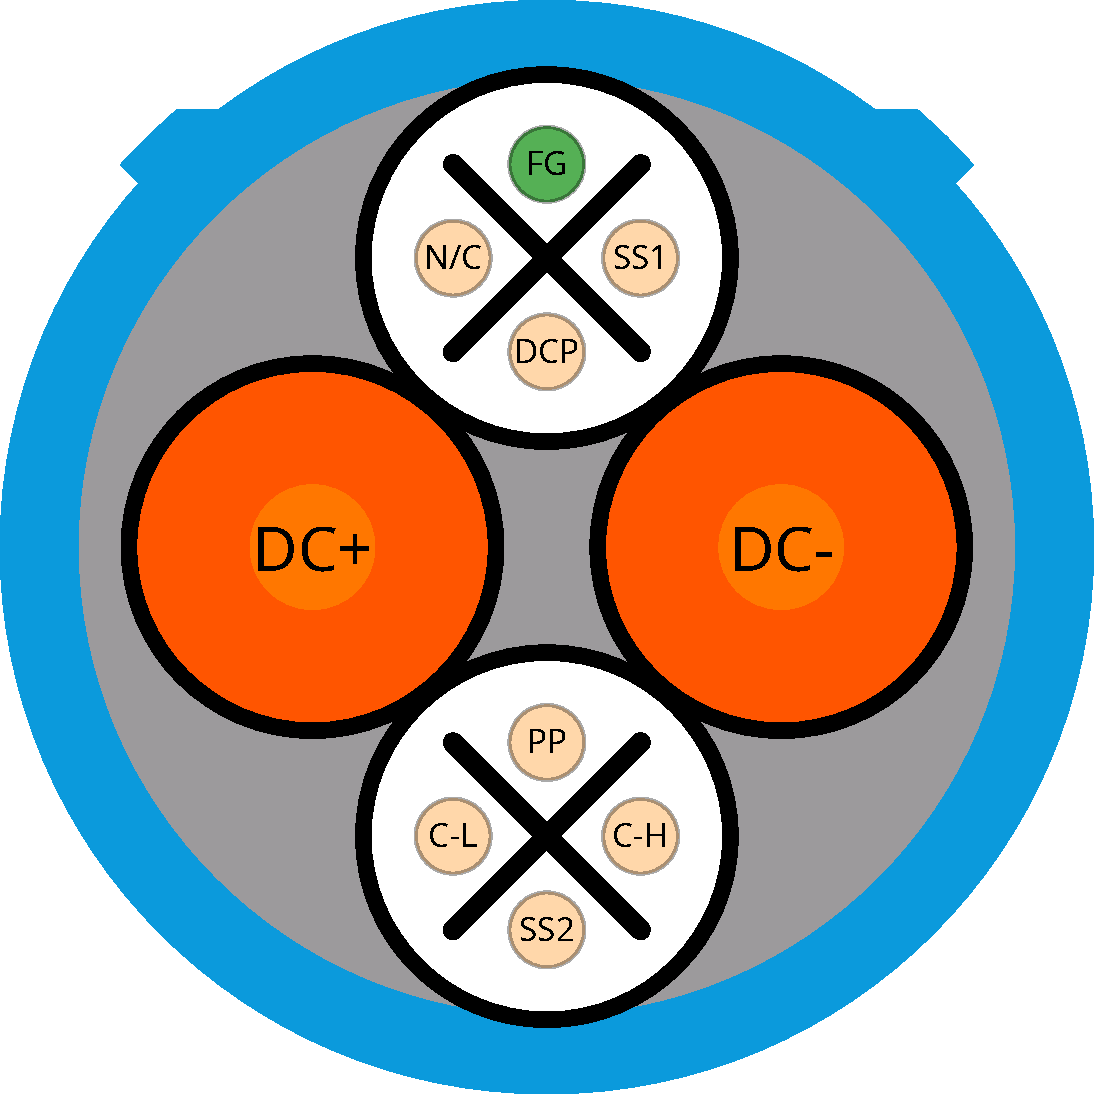
\includegraphics[width=.17\textwidth]{graphs/chademo}
        %\subcaption{Combined charging system connector schematic}
        \label{fig:ccs}
    \end{subfigure}
    \caption{Schematic diagrams of other fast charging connectors. From left to right: Type 1 CCS \cite{mliu92_drawing_2021}, NACS \cite{rickycourtney_drawing_2023}, MCS \cite{mliu92_speculative_2022}, GB-T \cite{mliu92_gbt-202343_2021}, Chademo \cite{mliu92_chademo_2021}}
    \label{fig:connectors}
\end{figure*}
% TODO add sources for all these images according to their creative commons licensing

% CCS1: By Mliu92 - Own work, CC BY-SA 4.0, https://commons.wikimedia.org/w/index.php?curid=108177318
% NACS: By RickyCourtney - Own work, CC BY-SA 4.0, https://commons.wikimedia.org/w/index.php?curid=133111353
% MCS: By Mliu92 - Own work, CC BY-SA 4.0, https://commons.wikimedia.org/w/index.php?curid=119080953
% GB/T: By Mliu92 - Own work, CC BY-SA 4.0, https://commons.wikimedia.org/w/index.php?curid=108206603
% chademo: By Mliu92 - Own work, CC BY-SA 4.0, https://commons.wikimedia.org/w/index.php?curid=108209697

\subsection{Other Communication Standards}
While Type 2 and CCS are the most used plugs for passanger cars in europe, there do exist some other plugs and charging standards for fast charging battery electric vehicles.
In total there are five other major plugs used for fast charging around the globe, listed below and shown schematically in \ref{fig:connectors}:

\begin{enumerate}
\item GB/T charging standard used in China
\item CHAdeMO used in Japan
\item Type 1 CCS formerly used in North America
\item NACS future north american charging standard
\item Megawatt charging system (MCS)
\end{enumerate}

While europe has the type 2 connector for three phase AC charging, america uses a different connector called type 1, since their power grid is usually not based on three phases.
There exists a type 1 CCS connector, adding two pins for DC charging, similarly to type 2 CCS.
Since communication is identical they can both be referred to as \enquote{CCS connectors}, or specified as \enquote{CCS1 connector} for the american version and \enquote{CCS2 connector} for the european version.
Similarly the megawatt charging system is also based on ISO15118, but uses a different connector, allowing higher currents and thus faster charging intended for trucks ans buses.
After Tesla open sourced their proprietary connector in 2022 \cite{noauthor_opening_nodate} it became quickly adopted by car manufacturers and charging station operators.
While its socket is different, it is also based on ISO15118 communication described above. \\
GB/T and CHAdeMO are the charging standards used in China and Japan respectively.
They use CAN bus for communication rather than powerline making their implementation easier and cheaper, while disallowing advanced use cases ISO15118 provides.
Since EV sales are much higher in Asia than in Europe and North America \cite{noauthor_trends_nodate}, the worldwide market share of vehicles with GB/T and CHAdeMO sockets remains significant nevertheless their usage only in China and Japan.
According to Blech \cite{blech_project_nodate} at the end of 2019 the combined market share of GB/T and CHAdeMO was 55\%. Figure \ref{fig:connector_marketshare} shows the market share of all connectors.

\begin{figure}[ht]
    \centering
    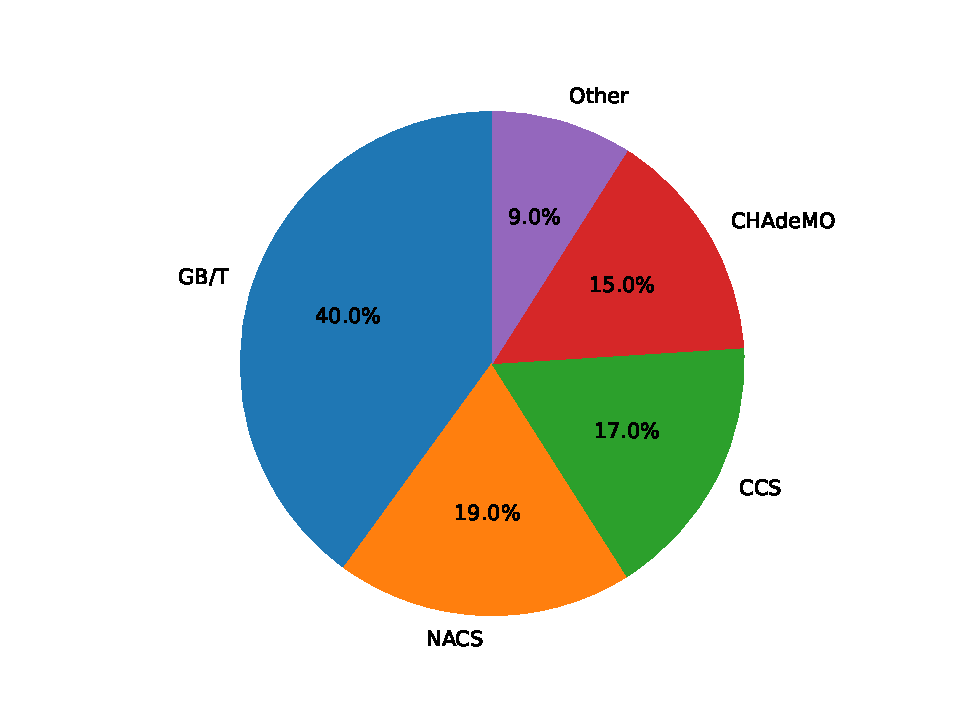
\includegraphics[width=.489\textwidth]{graphs/worldwide_plugs.pdf}
    \captionsource{Charging socket market share at the end of 2019}{Data based on Blech \cite{blech_project_nodate}.}
    \label{fig:connector_marketshare}
\end{figure}

%% \cite{dalheimer_ladeinfrastruktur_2017} - gonium talk about charging stations: TODO often other vulnerabilities
%% \cite{garofalaki_electric_2022} - OCPP security issues and challenges

\section{Charging station technologies and vendors}

\subsection{Charging station architectures}
% TODO: PV & battery storage integration
% ...

\subsection{Charging station market analysis}



%% \cite{das_electric_2020} - EV market share, charging standards list
%% TODO: add vendor market analysis
%% TODO: add charge port analysis
\begin{figure}[ht]
    \centering
    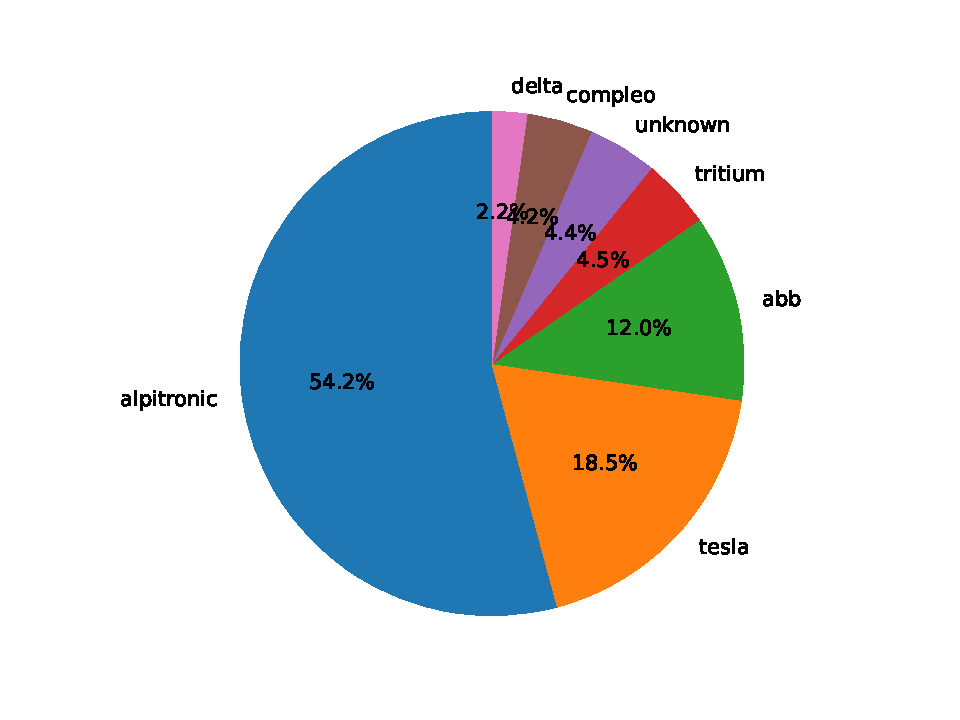
\includegraphics[width=.489\textwidth]{graphs/market_analysis.pdf}
    \caption{CCS charging station vendor market share}
    \label{fig:marketshare}
\end{figure}

\begin{figure}[ht]
    \centering
    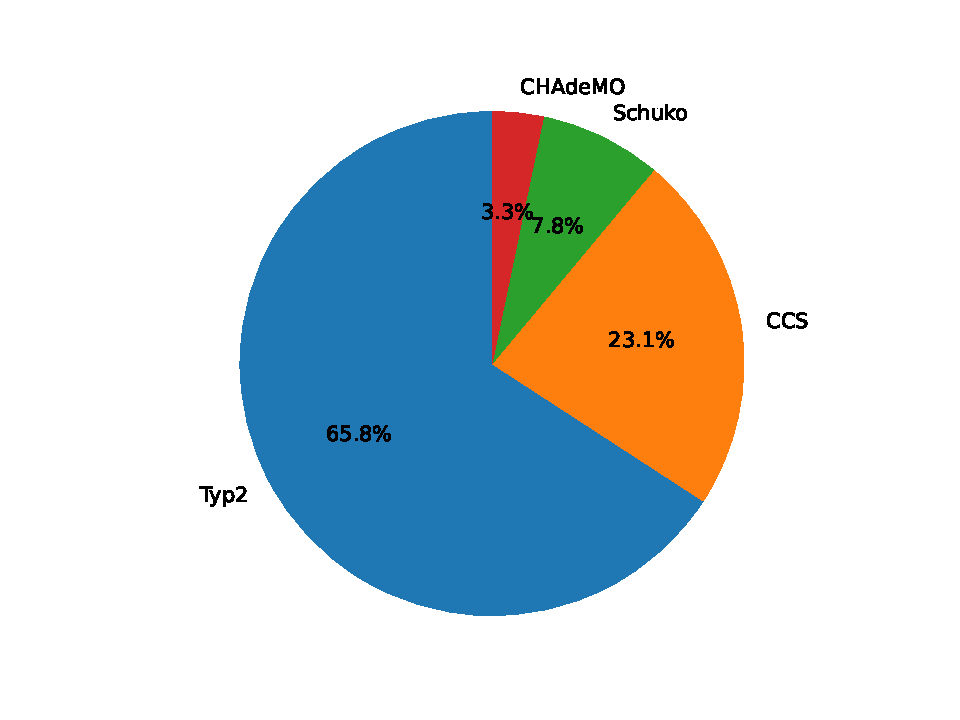
\includegraphics[width=.489\textwidth]{graphs/socket_analysis.pdf}
    \caption{Charging station socket market share}
    \label{fig:sockets}
\end{figure}

\begin{figure}[ht]
    \centering
    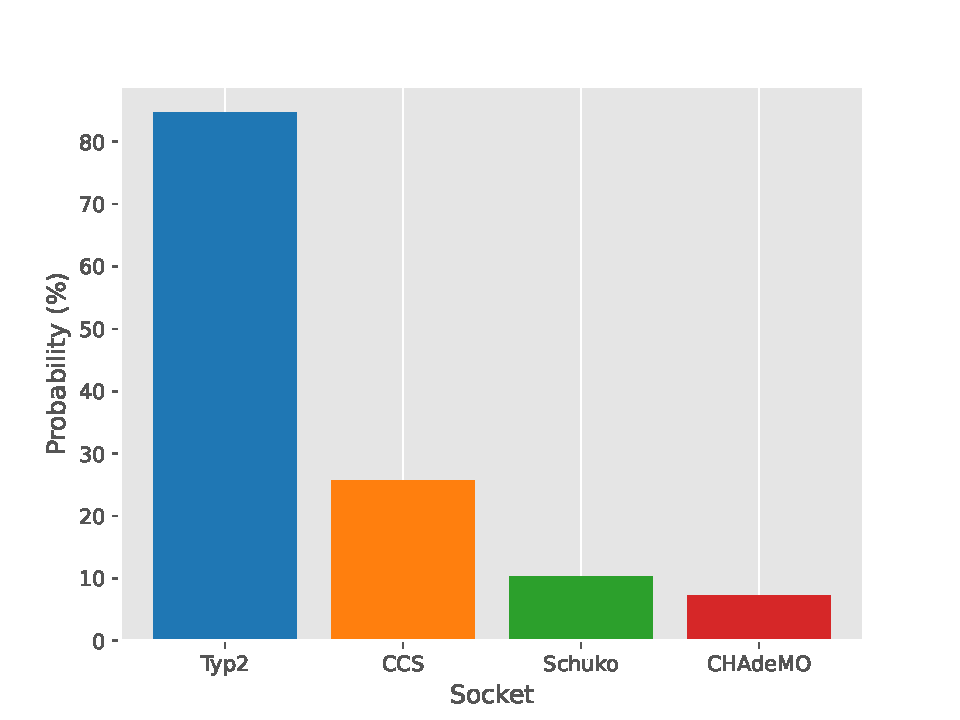
\includegraphics[width=.489\textwidth]{graphs/socket_probability.pdf}
    \caption{Probability to find socket X at a random charging location}
    \label{fig:socketsprob}
\end{figure}



\iffalse
\section{Charging Station Architectures}
% TODO: explain proposed architectures
%% \cite{acharya_cybersecurity_2020} - very good architecture schematic of grid/charging station/EV connections and communication.

\subsection{Proposed architectures}
%% \cite{deb_review_2021} - DC bus architektur
\subsection{Integration of battery storage and photovoltaics}
% TODO
\subsection{Independent charging stations}
% TODO: alpitronic
\subsection{DC Bus Systems}
% TODO: Tesla v4
\fi

\section{Attack Vectors and Impact}
%% \cite{bao_threat_2018} - ISO15118 threat analysis
%% \cite{kohler_brokenwire_2023} - jamming powerline in ISO15118 communication
%% \cite{nasr_chargeprint_2023} - framework for backend service security analysis

% impact:
%% \cite{sanghvi_cybersecurity_2021} - energy simulation using OpenDSS - impact of vulnerabilities
%% \cite{acharya_cybersecurity_2020} - very good architecture schematic of grid/charging station/EV connections and communication.

%% \cite{sklyar_chargepoint_nodate} - pentest of chargepoint charging station: many text-book vulnerabilities / buffer overflows / linux fails (suid bit, ssh rev tunnel to mothership, ...)

\iffalse
\section{Cybersecurity State}
\fi

\section{Conclusion}
While the market of both AC and DC charging stations is growing rapidly, as discussed in this paper, DC fast charging stations come with additional security implications.
Cybersecurity has not been a focus of the charging station industry in the past, leading to many text boot vulnerabilties in charging infrastructure.
In the recent past this situation is starting to improve, with various institutions publishing guidelines and plans on securing charging infrastructure \cite{mccarthy_cybersecurity_2023, encs_security_nodate}. \\
While this is a step in the correct directiona lot of low hanging fruits in regard to security research of DC charging stations remain untouched.
This is underlined by the fact, that most scientific publications covering cybersecurity of charging communication in general are purely theoretical.
While some AC charging stations and some web based services have been target of security research, little research has been done targeting real DC fast charging stations nor their communication with vehicles. \\
In future research our plan is to use automated pentesting techniques for identifying general problems with the ISO15118 standard and its implementations.


%% \cite{mccarthy_cybersecurity_2023} - NIST guidelines for IT security measures in EVs / charging stations / ... - as a recommendation?

\printbibliography
\end{document}
